\documentclass[printmode,openany]{mgr}
%opcje klasy dokumentu mgr.cls zostały opisane w dołączonej instrukcji

%poniżej deklaracje użycia pakietów, usunąć to co jest niepotrzebne
\usepackage{polski}
\usepackage[utf8]{inputenc}
\usepackage[T1]{fontenc}

%pakiety do grafiki
\usepackage{graphicx}
\usepackage{subfigure}
\usepackage{psfrag}
\usepackage{float}
\usepackage{pdfpages}

%pakiety dodające dużo dodatkowych poleceń matematycznych
\usepackage{amsmath}
\usepackage{amsfonts}

%pakiety wspomagające i poprawiające składanie tabel
\usepackage{supertabular}
\usepackage{array}
\usepackage{tabularx}
\usepackage{hhline}
\usepackage{booktabs}

%pakiet wypisujący na marginesie etykiety równań i rysunków
%zdefiniowanych przez \label{}, chcąc wygenerować finalną wersję
%dokumentu wystarczy usunąć poniższą linię
% \usepackage{showlabels}
\usepackage{url}
\usepackage{gensymb}

% własne makro
\newenvironment{breakparagraph}{\hfill\break}

%dane do złożenia strony tytułowej
\title{Optymalizacja procesu produkcji urządzeń elektronicznych}
\engtitle{Optimization of electronic devices manufacturing process}
\author{Mikołaj Guz}
\supervisor{dr hab. Mieczysław Wodecki}

\date{2019} %standardowo u dołu strony tytułowej umieszczany jest bieżący rok, to polecenie pozwala wstawić dowolny rok

%poniżej jest lista kierunków i specjalności na wydziale elektroniki,
%należy wybrać właściwe lub dopisać jeśli nie ma odpowiednich
\field{Automatyka i Robotyka (AIR)}
\specialisation{Technologie informacyjne w systemach automatyki (ART)}


%tutaj zaczyna się właściwa treść dokumentu
\begin{document}

\maketitle %polecenie generujące stronę tytułową

\tableofcontents %spis treści

\chapter{Wstęp}

W czasach coraz większej cyfryzacji życia potrzebna jest ogromna liczba różnego typu urządzeń elektronicznych.
W celu dostarczenia niezbędnych ilości należy spróbować usprawnić cały łańcuch produkcji elektroniki. Proces ten jest złożony i potrzeba odpowiednich narzędzi, żeby zmniejszyć czas produkcji, zminimalizować przestoje oraz podnieść jakość elementów końcowych. Jednym ze sposobów na to jest wyznaczanie optymalnych harmonogramów zadań, co jest kluczowym zadaniem w niniejsze pracy magisterskiej.

W tym dokumencie spróbujemy przeanalizować przykład produkcji elektroniki małoseryjnej oraz znaleźć rozwiązanie dla problemu przepływowego z przezbrojeniami.

\section{Cel i zakres pracy}
Celem pracy magisterskiej było stworzenie narzędzia do optymalizacji procesu produkcji urządzeń elektronicznych.
Aspektem badawczym pracy jest stworzenie modelu procesu produkcji oraz opracowanie algorytmów optymalizacyjnych na jego podstawie.
Aspekt inżynierski to zaprojektowanie odpowiednich algorytmów optymalizacyjnych oraz ich implementacja w oprogramowaniu. Aplikacja wykorzystana w pracy została stworzona\linebreak w języku C++ za pomocą bibliotek Qt.

\breakparagraph{}
Główne założenia pracy magisterskiej:
\begin{itemize}
	\item opis procesu produkcji,
	\item skonstruowanie modelu matematycznego dla danego problemu,
	\item implementacja algorytmów rozwiązujących dane zagadnienie,
	\item wykonanie badań,
	\item porównanie wyników.
\end{itemize}

\chapter{Opis procesu}

\section{Opis ogólny}
Proces badany w pracy to linia montująca płyty drukowane do finalnych produktów.
Sam proces składa się z kilku etapów:
\begin{enumerate}
	\item Pobranie potrzebnych elementów elektronicznych z magazynu.
	\item Uzbrojenie automatu pick\&place w wymagane elementy.
	\item Pobranie gotowych płyt PCB (ang. Printed Circuit Board).
	\item Ręczne nałożenie pasty lutowniczej za pomocą sitodruku
	\item Uruchomienie procesu montażu elementów na maszynie pick\&place.
	\item (Opcjonalnie) Umieszczenie ręczne elementów
	\item Przeprowadzenie procesu lutowania w piecu.
	\item (Opcjonalnie) Lutowanie ręczne.
	\item Kontrola gotowej płyty PCB\@.
\end{enumerate}

Cechy procesu:
\begin{itemize}
	\item wszystkie procedury muszą być wykonane w ustalonej kolejności,
	\item proces wymaga operatorów,
	\item dla płyt dwustronnych należy powtórzyć sekwencję,
	\item automat pick\&place może obsługiwać tylko jedną płytę PCB,
	\item piec lutowniczy może lutować kilka płyt drukowanych (ilość jest zależna od rozmiaru płyt).
\end{itemize}

Cały przepływ pracy został przedstawiony na diagramie~\ref{DiagFlow}.
Czerwone krawędzie wyznaczają ścieżkę krytyczną procesu.
Węzły o krawędziach przerywanych są to operacje opcjonalne zależne od projektu płyty PCB\@.

\begin{figure}[H]
	\centering
	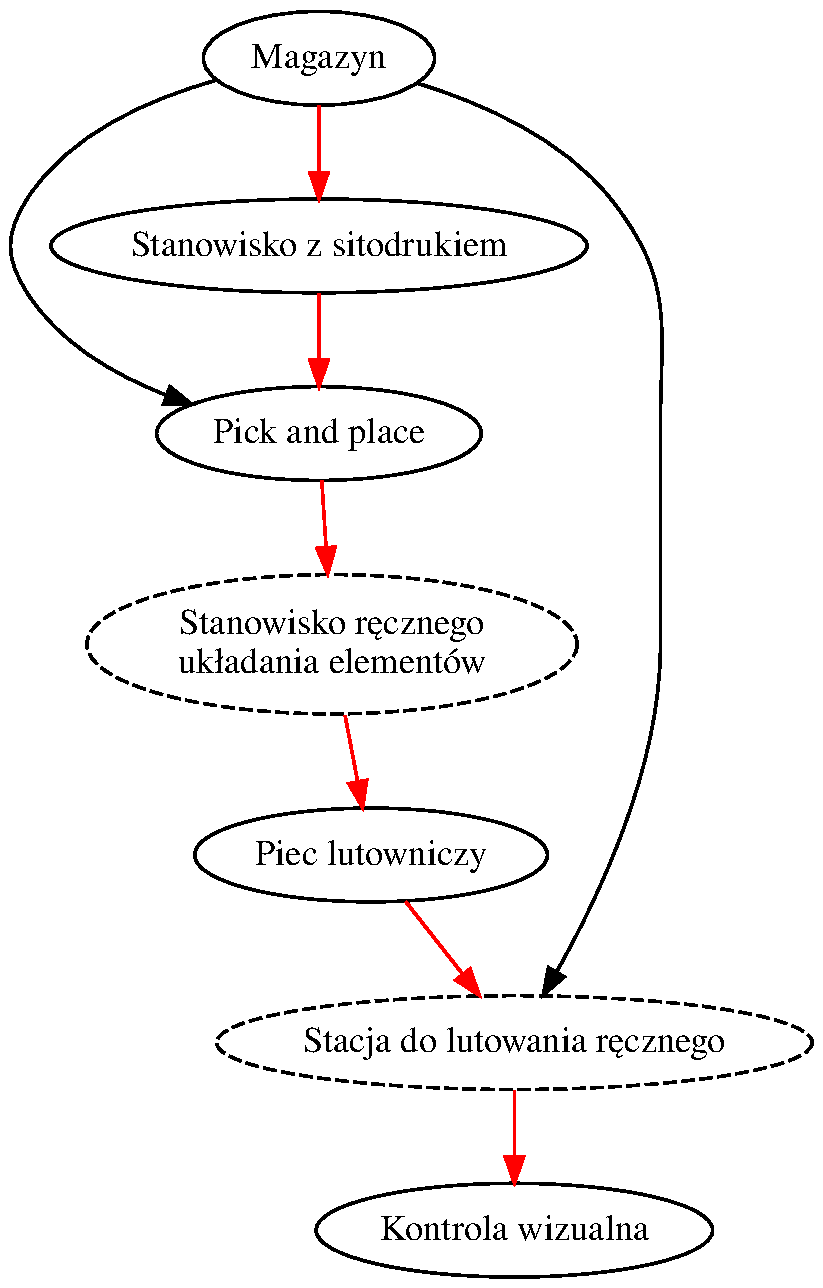
\includegraphics[scale=0.5]{./chapters/chapter2/flow_work.pdf}
	\caption{Diagram przepływu pracy w procesie}
	\label{DiagFlow}
\end{figure}

\section{Opis stanowisk}

\subsection{Magazyn}
Magazyn jest miejscem od którego zaczyna się cały proces.
Przechowuje on wszystkie niezbędne elementy elektroniczne (rezystory, kondensatory, układy scalone itd.), gotowe płyty PCB oraz szablony sitodruku do poszczególnych projektów.
Aktualny stan magazynowy oraz fizyczna lokalizacja produktów znajduję się w systemie ERP\@.
Wszystkie potrzebne przedmioty są pobierane przez operatora.

\subsection{Stanowisko z sitodrukiem}
W kolejnym etapie produkcji gotowa płytka PCB trafia na urządzenie sitodruku.
Możemy wyszczególnić kilka typów takiej maszyny~\cite{sitodruk}:
\begin{itemize}
	\item sitodruk manualny --- najprostsza wersja urządzenia. Cały proces sprowadza się do ręcznego ustawienia szablonu na płytce oraz ręcznego nałożenia pasty przez operatora. Cechuję się gorszą jakością i powtarzalnością operacji w porównaniu do urządzeń poniżej.
	\item sitodruk półautomatyczny --- operator ustawia płytkę względem szablonu często przy pomocy systemu wizyjnego. Proces naniesienia pasty odbywa się automatycznie. Rozwiązanie to często się wykorzystuje przy prototypowaniu oraz produkcji małoseryjnej.
	\item sitodruk automatyczny --- rola operatora sprowadza się do podania płytki i odebrania po naniesieniu pasty (system offline) lub załadowania podajnika czystymi płytkami i później odebraniu gotowych (rozwiązanie in-line). Wszystkie czynności takie jak ustawienie szablonu i nałożenie pasty odbywają się automatycznie.
\end{itemize}

W naszym przypadku używany jest sitodruk manualny (Rysunek~\ref{sitodruk}). Operator przed nałożeniem pasty na płytę PCB musi przezbroić maszynę. Proceder polega na przyniesieniu szablonu z magazynu oraz ustawieniu go na maszynie. W dalszym kroku następuje manualne naniesienie pasty.

\begin{figure}[H]
	\centering
	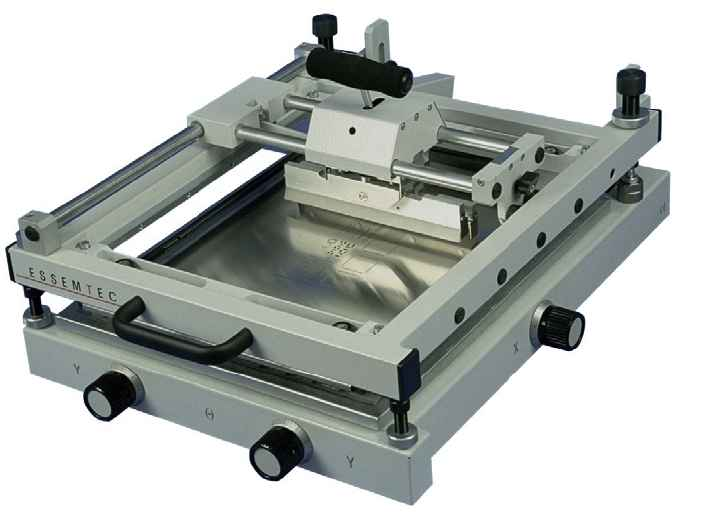
\includegraphics[scale=0.25]{./chapters/chapter2/sitodruk.jpg}
	\caption{Urządzenie sitodruku manualnego~\cite{sitodruk}}
	\label{sitodruk}
\end{figure}

\subsection{Automat pick\&place}
Automat pick and place to maszyna która umożliwia za pomocą systemu wizyjnego w precyzyjny sposób układać komponenty SMD na płytkach PCB~\cite{automatp&p1}. W procesie badanym wykorzystywany jest automat M10V firmy Mechatronika (Rysunek~\ref{automat_pick_place}). Średnia wydajność maszyny plasuję się na ok. 1200 --- 1600 komponentów na godzinę.

Cechy maszyny~\cite{automatp&p2}:
\begin{itemize}
	\item wbudowany system wizyjny,
	\item pełna automatyzacja nanoszenia elementów na płytę drukowaną,
	\item automatyczna korekcja na podstawie znaczników (ang.\ fiducials),
	\item korygowanie elementów na podstawie wykrycia złych oznaczeń na płycie,
	\item automatyczna zmiana dysz,
	\item automatyczne podawanie luźnych elementów (po wcześniejszej kalibracji),
	\item dane mogą pochodzić z różnych systemów danych CAD lub wprowadzane ręcznie w trybie TEACH-IN\@.
\end{itemize}

\newpage
Maszynę przed pracą z płytą PCB należy przezbroić. Operacja przezbrojenia polega na załadowaniu odpowiednich elementów elektronicznych oraz wykonaniu kalibracji.

Możliwe formy dostarczenia elementów do automatu:
\begin{itemize}
	\item taśmy 8 mm, 12 mm, 16 mm, 24 mm, 32 mm, 44 mm,
	\item tacki JEDEC,
	\item laski SO8–PLCC84,
	\item elementy luzem.
\end{itemize}

\begin{figure}[H]
	\centering
	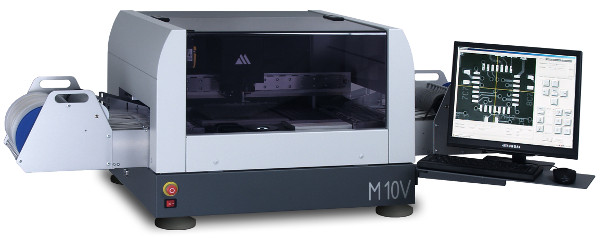
\includegraphics[scale=0.45]{./chapters/chapter2/M10V.jpeg}
	\caption{Automat M10V~\cite{automatp&p2}}
	\label{automat_pick_place}
\end{figure}


\subsection{Piec lutowniczy}
Piec lutowniczy to maszyna która umożliwia w procesie na technikę lutowania rozpływowego elementów SMD\@. Ważnym zagadnieniem przy lutowaniu rozpyłowym jest profil termiczny. Na podstawie profilu szacujemy czas trwania operacji na piecu.

Profil termiczny składa się z etapów:
\begin{description}
	\item[Etap 1] Nagrzewanie wstępne (preheat) --- wstępne nagrzewanie to wzrost temperatury z nachyleniem 1--3 \degree{C} do osiągnięcia około 150 \degree{C}. W tej fazie następuje częściowe odparowanie topnika.
	\item[Etap 2] Oczyszczanie (soak) --- aktywacja topnika umożliwiająca oczyszczenie chemiczne powierzchni złącza oraz usuniecie tlenków z stopu lutowniczego. Trwanie tego etapu to od 60 do 120 sekund.
	\item[Etap 3] Jednostajne rozgrzanie do rozpływu (ramp to peak) --- szybkie rozgrzanie mające na celu osiągnięcia temperatury likwidus (temperatura przemiany ciała stałego w ciekły) stopu lutowniczego.
	\item[Etap 4] Rozpływ (reflow) --- faza zasadnicza lutowania rozpływowego. Zachodzi w temperaturze od 215 do 250 \degree{C} (zależne od użytego stopu lutowniczego). W tym etapie stopiony stop tworzy połączenie pomiędzy polem lutowniczym a elementem elektronicznym. Czas trwania operacji to od 30 do 90 sekund.
	\item[Etap 5] Chłodzenie (cooling) --- ostatni etap polegający na możliwe szybkim schłodzeniu o nachyleniu 3--4 \degree{C}. Zbyt gwałtowne schłodzenie może spowodować naprężenie termiczne groźne dla elementów.
\end{description}

W procesie jest wykorzystywany piec eC-reflow-mate firmy Eurocircuits (Rysunek~\ref{piec}).

Specyfikacja pieca:
\begin{table}[H]
	\centering
	\begin{tabular}{cc}
		\toprule
		Maksymalny rozmiar płyty PCB & 350 $\times$ 250 mm                  \\\midrule
		Metody grzania                & promieniowanie IR, gorące powietrze \\\midrule
		Zakres temperatur             & Do 288 \degree{C}                    \\\midrule
		Komunikacja z komputerem      & USB                                  \\\midrule
		Wymiary                       & 520 $\times$ 620 $\times$ 245 mm     \\\midrule
		Waga                          & około 25 kg                         \\
		\bottomrule
	\end{tabular}
\end{table}

\begin{figure}[H]
	\centering
	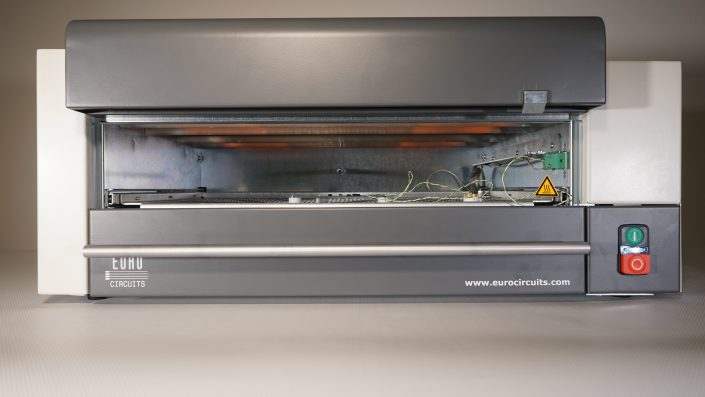
\includegraphics[scale=0.7]{./chapters/chapter2/piec.jpg}
	\caption{Piec lutowniczy}
	\label{piec}
\end{figure}

\subsection{Stanowisko do prac ręcznych}
Stanowisko to odpowiada w procesie za operacje operatora które przeprowadza ręcznie (ręczne nakładanie i lutowanie elementów oraz kontrolę wizyjną).

Stanowisko jest wyposażone w niezbędny sprzęt:
\begin{itemize}
	\item stację lutowniczą,
	\item stację hot-air,
	\item narzędzia drobne (szczypce, pęsety itd.),
	\item uchwyty montażowe,
	\item mikroskop.
\end{itemize}

\chapter{Sformułowanie problemu}
W tym rozdziale opiszemy przebieg rozpatrywanego procesu oraz przedstawimy jego model matematyczny.

% \section{Pare słów o Flow Shop}
% % ogarnij kolejność flow shop gdzie ma być
% \breakparagraph{}
% \textbf{Flow shop ($F_{m}$)} --- model $m$ pracujących maszyn i $n$ zadań. Każde zadaniem musi zostać obsłużone przez każdą maszynę. Kolejność operacji zadania jest ustalona z góry i nie ma możliwości jej zmiany. Dodatkowo zadanie nie może być przetwarzane przez kolejną maszynę, jeżeli nie zakończyło pracy na poprzedniej.


\section{Opis problemu}
Rozpatrywany problem jest to pewne uogólnienie klasycznego w teorii szeregowania permutacyjnego problemu przepływowego (ang. Flow-Shop). Dokładny opis tego problemu oraz algorytm metaheurystyczny jego rozwiązania są przedstawione między innymi w pracach ``Grabowski.J, Wodecki.M''~\cite{GRABOWSKI20041891} oraz ``Nowicki.E, Smutnicki.C''~\cite{NOWICKI1996160}

Dodatkowo w procesie występują przezbrojenia maszyn.

\breakparagraph{}
Ze względu na dużą złożoność procesu założone zostały pewne uproszczenia:
\begin{itemize}
	\item łańcuch transportu pomiędzy maszynami a magazynem został pominięty --- zakładamy, że potrzebne elementy znajdują przy każdym stanowisku,
	\item pomijamy ilość operatorów --- w pracy nie badamy wpływu ilości operatorów na czas trwania procesu, każda maszyna posiada własnego operatora,
	\item piec lutuje jednocześnie tylko jedną płytę PCB --- w warunkach rzeczywistych liczba lutowanych płyt PCB jest ograniczona powierzchnią roboczą pieca. Pominięcie tego założenia wymaga stosowania magazynów pomiędzy maszynami.0
\end{itemize}

\breakparagraph{}
Proces wytwarzania płyt jest realizowany na 6 stanowiskach (maszynach):
\begin{description}
	\item[Maszyna 1] Stanowisko z sitodrukiem manualnym.
	\item[Maszyna 2] Automat pick and place.
	\item[Maszyna 3] Ręczne układanie elementów.
	\item[Maszyna 4] Piec lutowniczy.
	\item[Maszyna 5] Stacja do lutowania ręcznego.
	\item[Maszyna 6] Kontrola wizyjna gotowych elementów.
\end{description}

\newpage{}
W procesie na 2 maszynach jest wykonywane przezbrojenie pomiędzy kolejnymi operacjami:
\begin{enumerate}
	\item Stanowisko sitodruku.
	\item Automat pick\&place
\end{enumerate}

\section{Model matematyczny procesu}

\breakparagraph{}
Zbiór maszyn
\begin{equation}
	M=\lbrace 1, 2, \dots, m \rbrace,
\end{equation}

gdzie $m$ to liczba maszyn. Maszyna reprezentuje stanowisko.

\breakparagraph{}
Zbiór zadań:
\begin{equation}
	J=\lbrace 1, 2, \dots, n \rbrace,
\end{equation}

gdzie $n$ to liczba zadań. Zadaniami są poszczególne płytki, które należy wykonać.

\breakparagraph{}
Zadanie $j \in J$ jest ciągiem $m$ operacji:
\begin{equation}
	O_{1, j}, O_{2, j}, \dots, O_{m, j},
\end{equation}

Operacja $O_{i,j}$ reprezentuje czynności, które należy wykonać na i-tej płytce na j-tym stanowisku.

\breakparagraph{}
Zmienne w modelu:
\begin{itemize}
	\item $p_{k, j}$ --- czas trwania operacji zadania $j$ na maszynie $k$
	\item $S_{k, j}$ --- moment rozpoczęcia operacji zadania $j$ na maszynie $k$
	\item $C_{k, j}$ --- moment zakończenia operacji zadania $j$ na maszynie $k$
\end{itemize}

\breakparagraph{}
Czas przezbrojenia pomiędzy zadaniem $i$ oraz $j$ na $k$-tej maszynie oznacza $s_{i, j}^{k}$, przez $( i \neq j \ oraz\ i, j \in J )$.

\breakparagraph{}
Łatwo zauważyć, że dowolne rozwiązanie problemu może być reprezentowane przez permutację zadania. Przez $\pi$ oznaczamy zbiór wszystkich permutacji elementów zbioru $J$.

Problem polega na wyznaczeniu minimalnego czasu zakończenia procesu. Muszą być przy tym spełnione następujące ograniczenia:
\begin{itemize}
	\item musi być zachowany porządek technologiczny operacji:
		  \begin{equation}
			  O_{1, j} \rightarrow O_{2, j} \rightarrow \dots \rightarrow O_{m, j}
		  \end{equation}
	\item każda operacja może być wykonywana tylko przez jedną maszynę,
	\item żadna maszyna nie może wykonywać więcej niż jednej operacji (uwagi: przypadek kiedy w piecu lutowniczym lutujemy jedną płytę PCB),
	\item wykonywanie żadnej operacji nie może zostać przerwane przed jej zakończeniem,
	\item momenty rozpoczęcia operacji oraz czas przezbrojenia nie mogą być ujemne:
		  \begin{equation}
			  S_{k, \pi(i)}, s^{k}_{\pi(i), \pi(j)} > 0
		  \end{equation}
\end{itemize}

Wprowadźmy następujące oznaczenia:
\begin{itemize}
	\item
	moment rozpoczęcia operacji $O_{i,\pi(j)}$:
	\begin{equation}
		S_{k, \pi(j)}=\max\{C_{k-1, \pi(j)}, C_{k, \pi(j-1)}+s^k_{\pi(j-1), \pi(j)}\},
	\end{equation}
	\item
	moment zakończenia operacji $O_{i,\pi(j)}$:
	\begin{equation}
		C_{k, \pi(j)} = S_{k, \pi(j)} + p_{k, \pi(j)},
	\end{equation}
	gdzie $ j \in J$ oraz $k \in M$.
\end{itemize}


\breakparagraph{}
Zakładamy przy tym, że moment rozpoczęcia procesu to:
\begin{equation}
	S_{1, \pi(1)}=0
\end{equation}

\breakparagraph{}
Zakończenie wszystkich zadań:
\begin{equation}
	C_{\max}(\pi) = 	C_{m, \pi(n)} = S_{m, \pi(n)} + p_{m, \pi(n)}
\end{equation}

\breakparagraph{}
W naszym przypadku optymalizacja procesu będzie polegała na wyznaczeniu optymalnej permutacji zadań $\pi^*$ takiej, że:
\begin{equation}
	C_{\max}(\pi^{*}) = \min\{C_{m, \pi{(n)}^{*}}\} \ \pi \in \Pi
\end{equation}

\chapter{Implmentacja programu}

\section{Przegląd zupełny}

\begin{figure}[H]
    \centering
    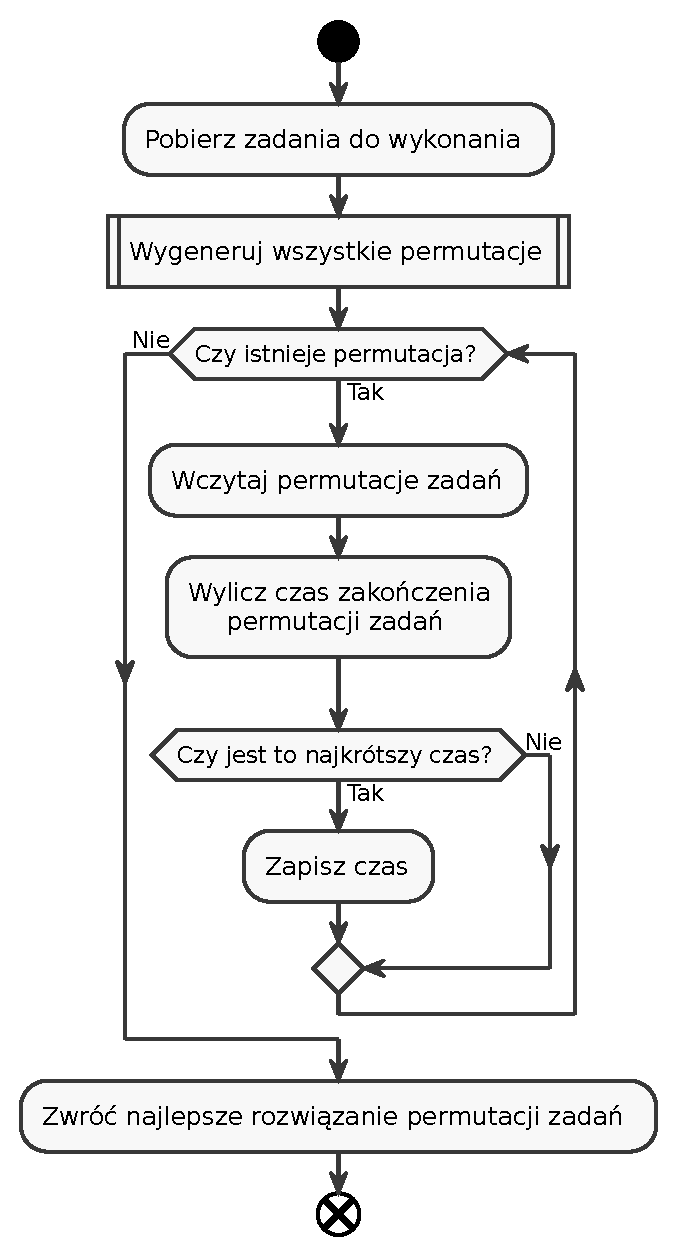
\includegraphics[scale=0.7]{chapters/chapter4/brute_force.pdf}
    \caption{Diagram algortmu "Przegląd zupełny"}
    \label{brute_force}
\end{figure}

\begin{figure}[H]
    \centering
    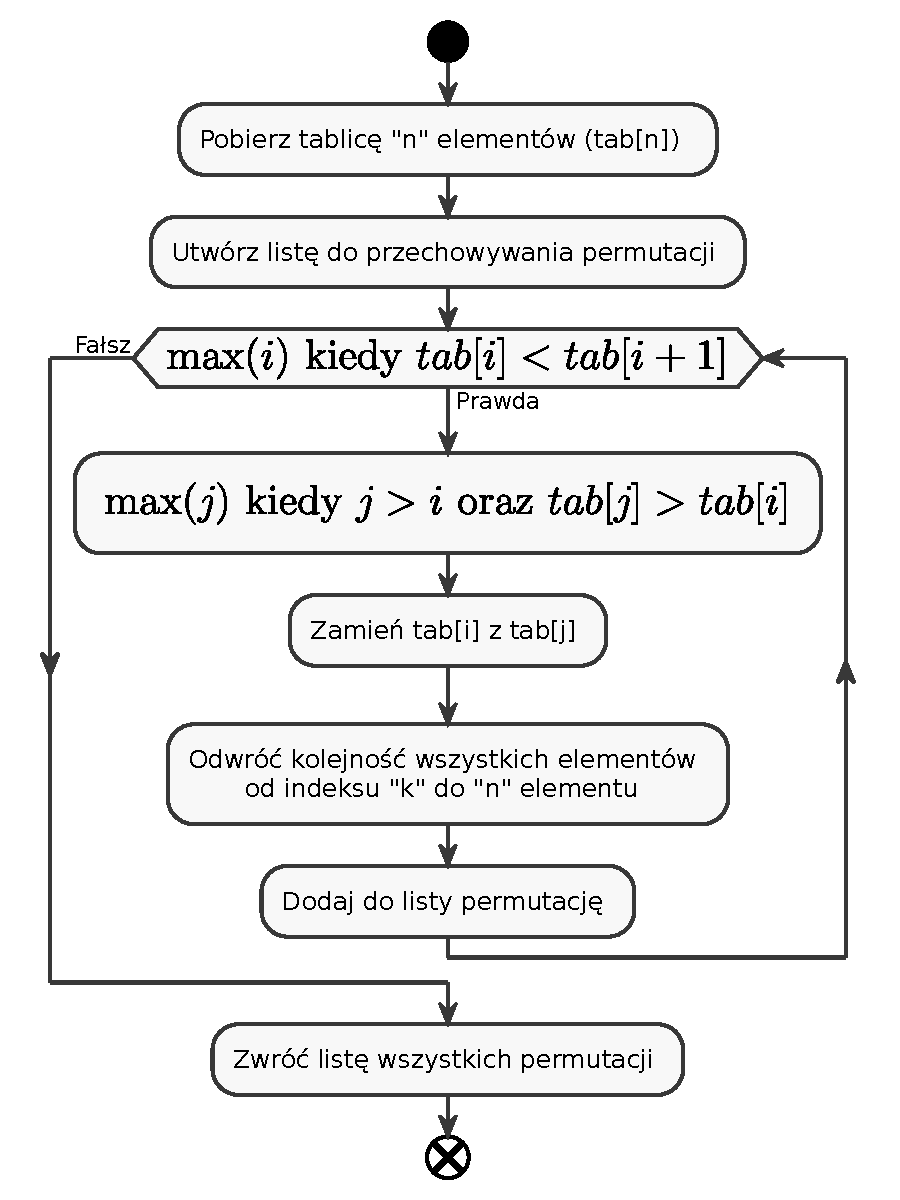
\includegraphics[scale=0.7]{chapters/chapter4/gen_perm.pdf}
    \caption{Diagram algorytmu "Porządek leksykograficzny"}
    \label{gen_perm}
\end{figure}
\section{Symulowane wyżarzanie}
\begin{figure}[H]
    \centering
    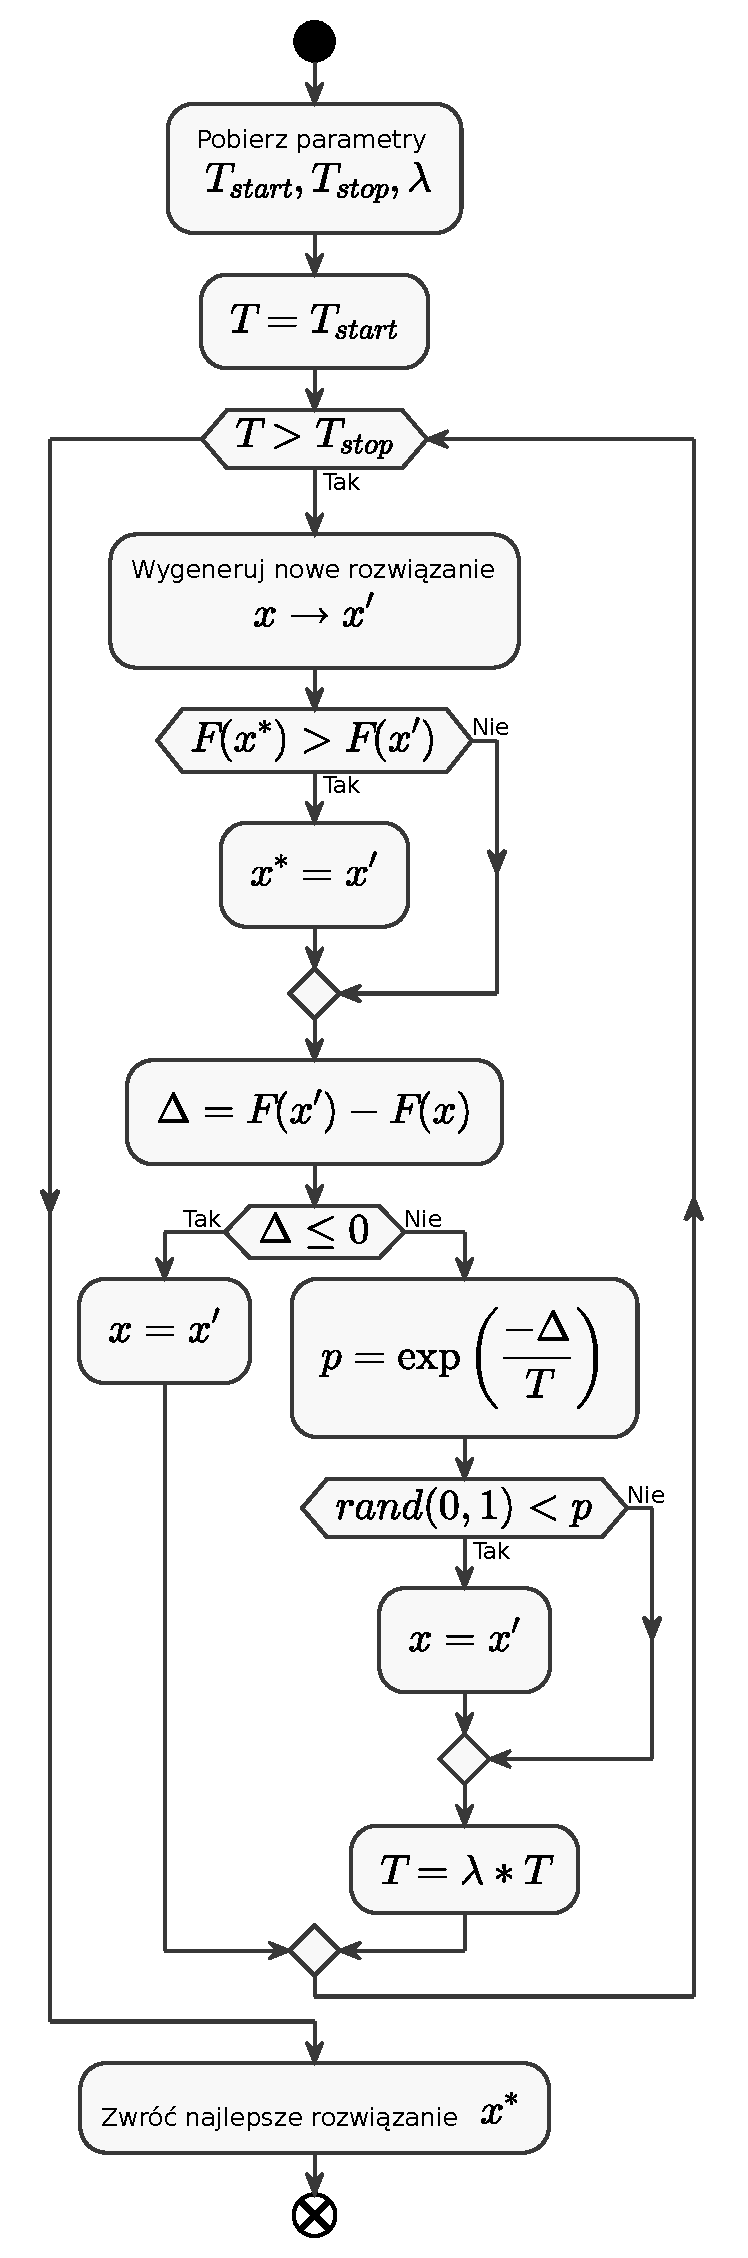
\includegraphics[height=\textheight]{chapters/chapter4/sa.pdf}
    \caption{Diagram algorytmu "Symulowane wyżarzanie"}
    \label{sa}
\end{figure}
\chapter{Badania}

\chapter{Podsumowanie}

Celem pracy magisterskiej było stworzenie narzędzia do optymalizacji procesu produkcji urządzeń elektronicznych. Zagadnieniem, jakie należało rozwiązać, był problem przepływowy z przezbrojeniem maszyn.

W pierwszym etapie przeanalizowano cały proces produkcji. Wyznaczono diagram przepływu pracy (Rysunek~\ref{DiagFlow}), dzięki czemu można było wyznaczyć ścieżkę krytyczną. Następnie przeanalizowano każde stanowisko pracy w celu znalezienia zależności procesowych oraz oceniono w jaki sposób można zoptymalizować pracę systemu.

Kolejnym etapem było sformułowanie problemu. Stworzony model pozwolił na zaobserwowanie, co jest wąskim gardłem w procesie produkcji oraz jakiego algorytmu należy użyć w celu optymalizacji.

W celu badań stworzono aplikację w C++. Użyto do tego bibliotek i narzędzi w Qt. Umożliwia to w przyszłości dodawanie nowych funkcjonalności do programu, np. interfejsu graficznego. W projekcie wykorzystano również bazę danych SQLite. Dzięki temu w sposób spójny można dostarczyć do aplikacji potrzebne dane o poszczególnych projektach.

Następnie wybrano dwa algorytmy do rozwiązania problemu przepływowego z przezbrojeniami: przegląd zupełny oraz symulowane wyżarzanie. Przegląd zupełny to algorytm dokładny. Oznacza to, że otrzymane rozwiązanie jest zawsze optymalne, lecz jak dowiodły badania, okupione dużą złożonością obliczeniową. Stwarza to możliwość wyznaczenia optymalnej permutacji zadań, w celu porównania z rozwiązaniami przybliżonymi. Symulowane wyżarzanie to algorytm z grupy metaheurystycznych. Znajduje on rozwiązanie przybliżone w dość krótkim czasie.

Z badań wynika, że SA jest algorytmem szybkim i dającym dość dobre wyniki. Jego wadą jest silnie sparametryzowanie, więc należy dużą uwagę poświęcić na odpowiednie dobranie parametrów. Kolejnym wnioskiem jest, że przegląd zupełny nie nadaje się do dużych zbiorów zadań ($n>11$). Czas wykonania drastycznie się wtedy zwiększa, przez co jego przydatność jest mała.

Jak można zauważyć, optymalizacja procesu rzeczywistego jest dość trudnym zadaniem. W pracy omawiany jest przypadek z dużą ilością uproszczeń oraz małą ilością maszyn. W warunkach przemysłowych produkcji elektroniki, gdzie maszyn jest kilkadziesiąt, problem staje się bardziej złożony. W tej sytuacji nie można pozwolić na jakiekolwiek uproszczenia, przez co należy użyć bardziej wyrafinowanych technik optymalizacji.

\addcontentsline{toc}{chapter}{\bibname} %utworzenie w spisie treści pozycji Literatura

\raggedright{
	\bibliography{bibliography} % wstawia bibliografię korzystając z pliku
	\bibliographystyle{ieeetr} %tylko gdy używamy BibTeXa, ustawia polski styl bibliografii
}

%opcjonalnie może się tu pojawić spis rysunków i tabel
% \listoffigures
% \listoftables
\end{document}
